%% Direttive TeXworks:
% !TeX root = ./presentazione.tex
% !TEX encoding = UTF-8 Unicode
% !TEX program = arara
% !TEX TS-program = arara
% !TeX spellcheck = it-IT

%! arara: clean: { files: [ arara.log, presentazione.aux, presentazione.log, presentazione.nav, presentazione.out, presentazione.snm, presentazione.toc, presentazione.xmpdata, pdfa.xmpi ] }
% arara: clean: { files: [ arara.log, presentazione.log ] }
% arara: pdflatex: { synctex: yes, action: batchmode, options: "-halt-on-error -file-line-error-style" }
% arara: pdflatex: { synctex: yes, action: nonstopmode, options: "-halt-on-error -file-line-error-style" }

%% Genera un file report.xmpdata con i dati di titolo e autore per il formato PDF/A %%
\begin{filecontents*}{\jobname.xmpdata}
\Title{Kotlin / JavaScript}
\Author{Luca Semprini}
\Copyright{Copyright \copyright 2018, Luca Semprini}
\Keywords{Kotlin\sep Code\sep JavaScript\sep JS}
\end{filecontents*}
\documentclass{beamer}

%% ORDINE IMPORTANTE INIZIO %%%%%%%%%%%%
\usepackage[T1]{fontenc}        % serve per impostare la codifica di output del font
\usepackage{textcomp}           % serve per fornire supporto ai Text Companion fonts
\usepackage[utf8]{inputenc}     % serve per impostare la codifica di input del font
\usepackage[
    english,        % utilizza l'inglese come lingua secondaria
    italian         % utilizza l'italiano come lingua primaria
]{babel}                        % serve per scrivere Indice, Capitolo, etc in Italiano
\usepackage{lmodern}            % carica una variante Latin Modern prodotto dal GUST
%% ORDINE IMPORTANTE FINE %%%%%%%%%%%%%%

\usepackage{xcolor}             % serve per la gestione dei colori nel testo
\usepackage{graphicx}           % serve per includere immagini e grafici

\usepackage[%
    strict,             % rende tutti gli warning degli errori
    autostyle,          % imposta lo stile in base al linguaggio specificato in babel
    english=american,   % imposta lo stile per l'inglese
    italian=guillemets  % imposta lo stile per l'italiano
]{csquotes}                     % serve a impostare lo stile delle virgolette

\setcounter{secnumdepth}{2}     % Numera fino alla sottosezione nel corpo del testo
\setcounter{tocdepth}{3}        % Numera fino alla sotto-sottosezione nell'indice

\graphicspath{{img/}}

\usepackage[%
    depth=3,            % equivale a bookmarksdepth di hyperref
    open=false,         % equivale a bookmarksopen di hyperref
    numbered=true       % equivale a bookmarksnumbered di hyperref
]{bookmark}                     % Gestisce i segnalibri meglio di hyperref
\usepackage{hyperref}           % Gestisce tutte le cose ipertestuali del pdf
\hypersetup{%
    pdfpagemode={UseNone},
    hidelinks,          % nasconde i collegamenti (non vengono quadrettati)
    hypertexnames=false,
    linktoc=all,        % inserisce i link nell'indice
    plainpages=false,
    breaklinks,
    bookmarks=true,
    pdfstartview={Fit},
    unicode=true,       % only Latin characters in Acrobat's bookmarks
    pdftoolbar=false,   % show Acrobat's toolbar?
    pdfmenubar=false,   % show Acrobat's menu?
    plainpages=false
}
\usepackage[pdf15,a-1b]{pdfx}

\usetheme{Boadilla}             % serve per scegliere il layout generale dei frame
\usecolortheme{beaver}          % Per il colore va comunque bene questo
\setbeamerfont{block title}{size=\normalsize}
\setbeamerfont{block body}{size=\small}

%% Permette di inserire l'outline prima di ogni sezione
\AtBeginSection[]{%
    \begin{frame}<beamer>
        \frametitle{Outline}
        \tableofcontents[currentsection]
    \end{frame}
}

\title[KotlinJs]{%
    KotlinJS
}
\subtitle{Compiling Kotlin to JavaScript}

\author[Luca~Semprini]{\large{Luca~Semprini}\\\medskip\small{0000854447}}

% \date{30 maggio 2018}
% \institute[]{%
    % Alma Mater Studiorum - Università di Bologna\\%
    % Campus di Cesena%
% }
% \titlegraphic{\includegraphics{Rx_Logo}}

\date[30 maggio 2018]{}
\institute[]{%
    
\includegraphics[scale=0.33]{kotlin2jsLogo}\\%
    \bigskip%
    \small{%
        Alma Mater Studiorum - Università di Bologna\\%
        Campus di Cesena%
    }
}

\begin{document}
    \begin{frame}
        \titlepage
    \end{frame}
    \begin{frame}
      \tableofcontents
    \end{frame}

    \section{Introduzione}
    \begin{frame}
      \frametitle{Kotlin: di cosa si tratta}
        \begin{block}{Definizione}
          Linguaggio di programmazione Object-Oriented \alert{staticamente tipizzato} e
          prevalentemente improntato su Java (JVM).
        \end{block}

        \bigskip

        \begin{block}{Un po' di storia}
          \begin{itemize}[<+->]
            \item Nasce nel 2011 da un team di sviluppatori di JetBrains.
            \item 15 febbraio 2016: Rilascio della versione 1.0.
            \item Dal 17 maggio 2017 linguaggio \alert{ufficiale} per Android.
          \end{itemize}
        \end{block}
    \end{frame}

    \begin{frame}
      \frametitle{L'Obiettivo? Sostituire Java}
      \begin{center}
        
\includegraphics[scale=0.33]{img/KotlinMeme}
      \end{center}
    \end{frame}

    \begin{frame}
      \frametitle{I Pilastri della Filosofia di Kotlin}
      \begin{block}{Pragmatismo}
        \begin{itemize}
          \item Accorpare funzionalità e soluzioni affidabili e di successo.
          \item Integrazione di O-O e Funzionale: $tipi$ $funzionali$.
        \end{itemize}
      \end{block}
      \begin{block}{Concisione}
        Ampia riduzione del Boilerplate Java, sintassi più snella.
      \end{block}
      \begin{block}{Sicurezza}
        Tutti i vantaggi della tipizzazione statica, più la \textbf{\alert{Null Safety}}: marcare i tipi come $nullable$.
      \end{block}
      \begin{block}{Interoperabilità (senza sforzo)}
        \begin{itemize}
          \item Si basa completamente sulle classi di standard library di Java, estendendole.
          \item Bytecode è compatibile con Java.
          \item Tool convertitore Java-to-Kotlin e Kotlin-to-Java.
        \end{itemize}
      \end{block}
    \end{frame}

    \begin{frame}
      \frametitle{Hello Kotlin!}
      Un esempio di Hello World:
      \begin{center}
        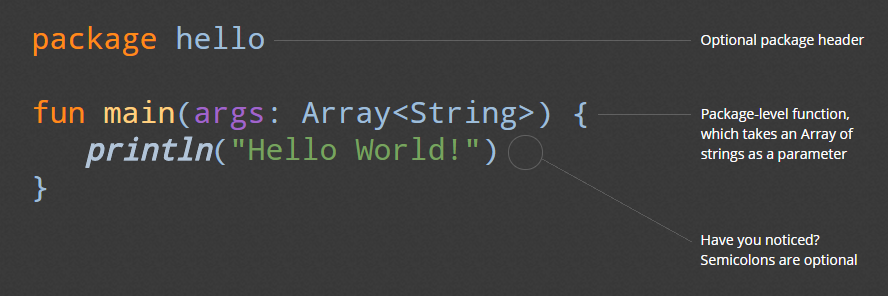
\includegraphics[scale=0.5]{img/HelloWorld}
      \end{center}
    \end{frame}
\end{document}
